\chapter{Modellazione e gestione statica di un cluster di nove incroci interconnessi}
In questo terzo capitolo viene presentato il modello utilizzato per la simulazione di un cluster di nove incroci interconnessi. Tutti questi incroci sono a raso a quattro bracci, esattamente come la singola giunzione vista in precedenza, ma la particolarità è che, essendo collegati, i veicoli che fluiscono da un incrocio entreranno a far parte di una delle code di uno degli incroci successivi. In questo modo si vuole analizzare se una gestione dinamica, come quella presentata, effettivamente riesca ad apportare dei benefici in un contesto più ampio di quello della singola intersezione, o se, al contrario, efficientare il flusso di veicoli di una giunzione congestiona pesantemente le altre.

La base di partenza è, ovviamente, il modello del singolo incrocio realizzato ed ampiamente commentato in precedenza, che è stato trasformato in un sottosistema. Materialmente lo si è inserito in un blocco \textit{Subsystem}\cite{subsystem}, anche questo già visto in precedenza, ed al posto degli \textit{Entity Generator}, sono state collegate alle code delle \textit{Input Port}.

Anche i terminator sono stati eliminati dal blocco, sostituiti invece da delle \textbf{Output Port \cite{outputport}}. Tutto questo è stato fatto in modo tale da poter interconnettere gli incroci: queste porte sono infatti poi accessibili dall'esterno del \textit{Subsystem}, in modo tale da far passare le entità da un sottosistema (e dunque da un incrocio) ad un altro.

\begin{figure}[H]
\centering
  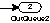
\includegraphics[width=0.3\textwidth]{OutputPort.pdf}
  \caption{Output Port}
  \label{fig:}
\end{figure}

Resta fondamentale sottolineare la presenza di un \textbf{Entity Output Switch \cite{switch}} prima delle \textit{Output Port} di quelle corsie che permettono alle automobili presenti all'interno delle stesse sia di andare dritto che di svoltare a destra. Infatti, se è vero che in precedenza non era importante la decisione presa, in quanto riguardava solo l'uscita dal singolo incrocio, in questo caso invece è fondamentale capire quando un'auto "decide" di proseguire dritto o, al contrario, di girare, perché quella stessa vettura poi, a seconda della sua decisione, proseguirà verso un'altra intersezione specifica. 

Per implementare questo meccanismo decisionale ci si è avvalsi, appunto, di un \textit{Entity Output Switch}. Quello che fa questo componente è molto semplice: per ogni entità che lo attraversa, decide secondo un criterio stabilito (una distribuzione o una funzione) su quale porta di output inviarla. Il numero di canali di output viene precedentemente specificato, così come il meccanismo di scelta. 

\begin{figure}[H]
  \includegraphics[width=1\textwidth]{switchEproprieta.pdf}
  \caption{Entity Output Switch e relativa configurazione}
  \label{fig:}
\end{figure}

In questo caso, come si può notare dalla figura precedente, le output ports sono ovviamente due, una relativa all'uscita che collega tale corsia con l'incrocio immediatamente di fronte ad essa (l'automobile ha deciso di proseguire diritto), un'altra inerente al collegamento con la giunzione a destra rispetto alla corsia designata (l'auto ha deciso di svoltare).

La scelta viene effettuata casualmente in maniera equiprobabile e se ne occupa l'Entity Switch stesso. Come spesso accade in informatica, tuttavia, la decisione viene associata alla generazione di un numero casuale, tramite il quale il componente si regola in autonomia. La generazione di questo numero ha bisogno di un Seed, ovvero un altro numero di partenza, questa volta però predeterminato, ovvero dato in input come parametro all'Entity Switch.

In sostanza, in base a questo numero il componente prenderà una decisione per ogni veicolo che lo attraversa. Questo però espone il modello ad un problema: se il Seed fosse sempre lo stesso anche i numeri generati casualmente in realtà sarebbero identici per ogni simulazione, e quindi se è vero che all'interno della stessa simulazione la scelta sarebbe casuale, è anche vero che fra due simulazioni consecutive in realtà il meccanismo sarebbe deterministico, in quanto si potrebbe già sapere che strada prenderà ciascun veicolo, sulla base del comportamento precedente.

Per spiegarsi meglio, ecco un esempio molto banale: nella ipotetica \textbf{Simulazione A} il \textit{Veicolo 1} della corsia che si sta prendendo in considerazione sceglie di andare dritto. Questo non fornisce alcuna informazione sulla decisione che  prenderà il \textit{Veicolo 2}, e quindi sembra che tutto sia casuale. Si ipotizzi che il \textit{Veicolo 2} decida di svoltare a destra.

In una futura \textbf{Simulazione B}, però, se il Seed inerente a quello specifico Entity Output Switch non è cambiato, si avrà la matematica certezza che il \textit{Veicolo 1} sceglierà di proseguire dritto, e che il \textit{Veicolo 2}, invece, svolterà. Questo rappresenta ovviamente un problema, perché si vuole rendere il modello assolutamente casuale, in modo tale da poter effettuare simulazioni diverse fra loro per validare l'ipotesi per cui una gestione dinamica è valida anche in questo tipo di ambiente.
\newline

Per risolvere il problema, i Seed di ogni Entity Output Switch sono stati generati casualmente all'avvio della simulazione, utilizzando questa volta la funzione \textit{Randi} messa a disposizione da Matlab, inserita nella sezione InitFcn del modello (si veda la \textit{figura \ref{fig:initfcn}}).
Il codice utilizzato è il seguente.
\newline
\begin{lstlisting}[language=Matlab,label=seedgen,caption=Generazione Casuale dei Seed]
    coder.extrinsic('randi');
	seeds = 1;
	seeds = randi(10000, [1 44]); 
\end{lstlisting}

In definitiva, il modello della singola corsia (dritto / destra) è quello in figura. Come si può notare non è stato cambiato nulla che non sia stato citato in questa sua breve descrizione. 

\begin{figure}[H]
  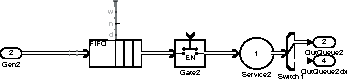
\includegraphics[width=1\textwidth]{catenaIncrocioModificato.pdf}
  \caption{Singola corsia (dritto / destra) di una giunzione del cluster}
  \label{fig:}
\end{figure}

\newpage
\section{La modellazione del cluster}
Compresi i cambiamenti che sono stati apportati al modello del singolo incrocio, è bene descrivere come si è creato il cluster delle nove giunzioni interconnesse.

In primo luogo, ogni sottosistema dispone, ovviamente, di otto porte di input, corrispondenti alle otto corsie dell'incrocio, e di dodici porte di output. In \textit{figura \ref{fig:switchstreet}} si può notare che sono stati utilizzati degli \textbf{Entity input switch \cite{inpswitch}}, elementi leggermente diversi dagli \textit{Entity Output Switch}, in quanto presentano un numero di ingressi multiplo ed un'unica uscita. Essi sono stati poi collegati a degli \textit{Output Switch}.

\begin{figure}[H]
\centering
  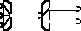
\includegraphics[width=0.5\textwidth]{switchStreet.pdf}
  \caption{Collegamento fra Entity Input Switch ed Entity Output Switch}
  \label{fig:switchstreet}
\end{figure}

Questo per un motivo molto semplice: considerando due incroci adiacenti, A e B, ci sono tre corsie di uscita da A che vanno verso B, e solo due ingressi per B (quelli del braccio collegato ad A). Un'analisi della \textit{figura \ref{fig:ingrandimentoincroci}} è più esplicativa di mille parole. 

Prendendo per esempio proprio la figura seguente, si chiami A l'incrocio più a sinistra e B quello più a destra. Le corsie di uscita da A che vanno verso B sono:
\begin{enumerate}
  \item Braccio Nord - Corsia per svoltare a sinistra
  \item Braccio Sud - Corsia per svoltare a destra
  \item Braccio Ovest - Corsia per andare dritto
\end{enumerate}
Mentre per quanto concerne le corsie di B che sono collegate ad A, queste sono solo quelle del braccio Ovest, quella per andare dritto / svoltare a destra e quella per svoltare a sinistra.
\begin{figure}[H]
  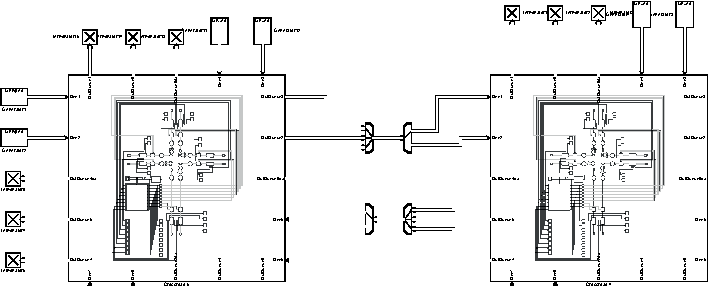
\includegraphics[width=1\textwidth]{collegamentoIncroci.pdf}
  \caption{Ingrandimento del raccordo fra due incroci adiacenti}
  \label{fig:ingrandimentoincroci}
\end{figure}

Ecco dunque spiegata l'utilità degli Switch, che servono a redistribuire i veicoli provenienti da A nelle corsie di B adiacenti, anche questa volta utilizzando un Seed generato casualmente per ogni esecuzione. Ogni \textit{Input Switch}, nello specifico, si occupa di accorpare il flusso di autovetture provenienti dalle tre corsie di output di un incrocio, e di inviare questo flusso ad un \textit{Output Switch}, che smista le automobili nelle due strade di input dell'incrocio successivo.
\newline

Ovviamente queste automobili devono essere in qualche modo generate, e devono in qualche modo fuoriuscire dal cluster. Per questo gli incroci più esterni, in alcune delle loro corsie, sono stati collegati a degli Entity Generator, programmati esattamente come visto per il modello a singolo incrocio, e a degli Entity Terminator. È palese che la struttura creata sia frattalica ed ampiamente espandibile: nulla impedisce di creare un cluster di un numero di incroci nettamente superiore a nove, ma lo scopo di questa tesi non è quello di mappare le intersezioni stradali di un'intera città in un modello di SimEvents.

È anche importante notare che in questo caso la capacità delle code che rappresentano le corsie non è stata lasciata ad infinito, essendo in realtà rappresentativa della distanza fra due giunzioni consecutive. Pertanto si è deciso di operare in questo modo: le code direttamente collegate a degli \textit{Entity Generator} sono state volontariamente programmate per avere lunghezza infinita, in quanto altrimenti si sarebbero potute riempire in situazioni di traffico intenso non dando la possibilità ai generator di funzionare a dovere. Per quelle che invece rappresentano una corsia che collega un incrocio ad un altro, la loro capienza è stata impostata ad un numero massimo, il cui valore specifico sarà poi reso noto nel paragrafo relativo alle simulazioni effettuate.

In definitiva, il modello a nove incroci è presentato nella figura seguente.
\newpage

\begin{figure}[H]
  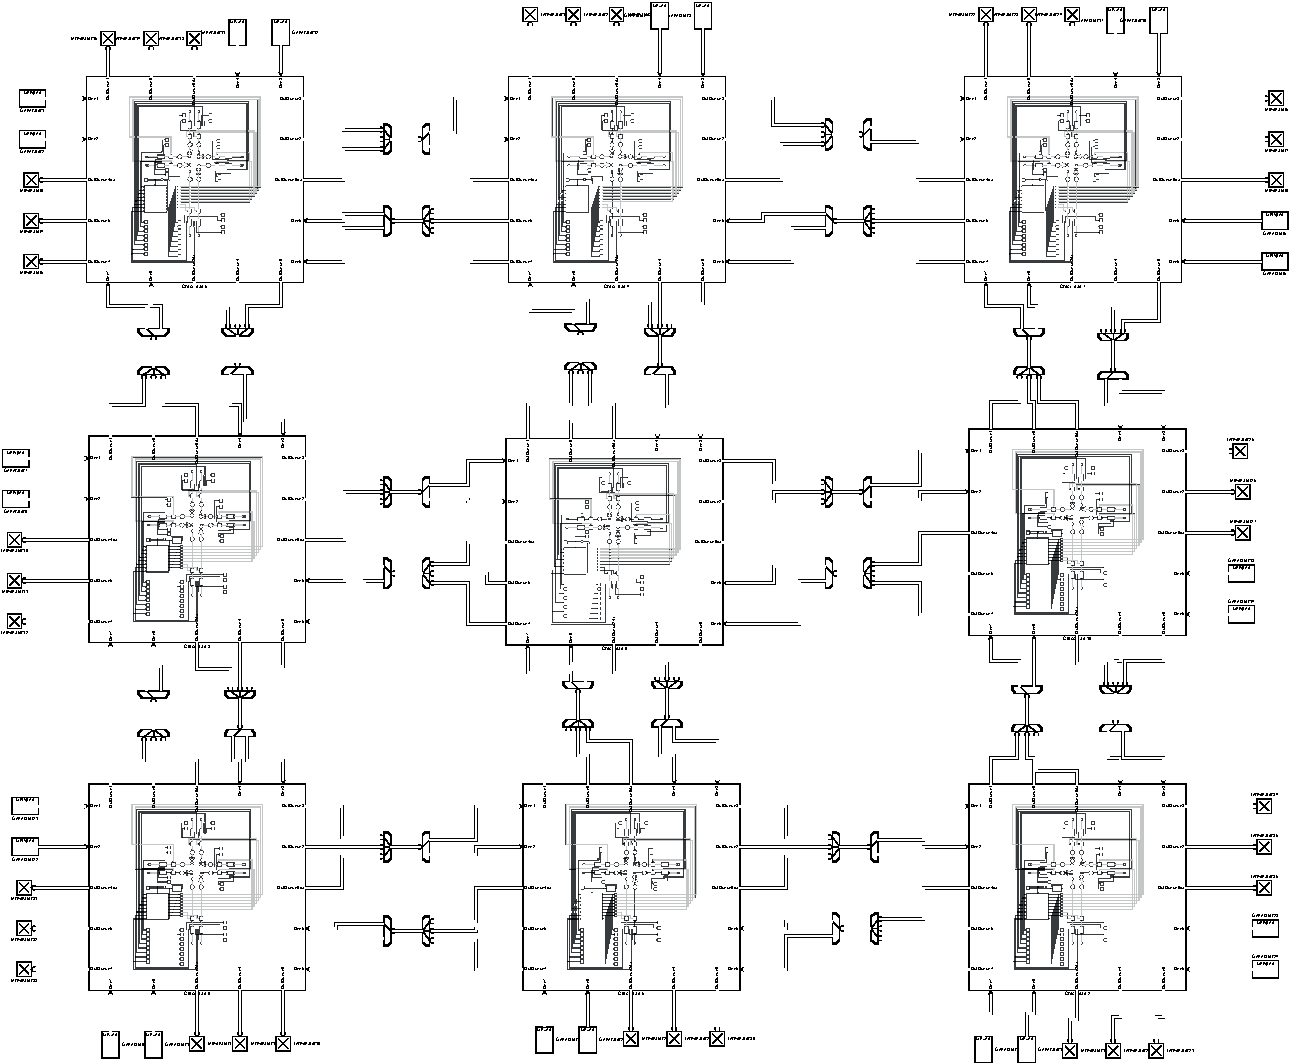
\includegraphics[width=1\textwidth]{capitolo3.pdf}
  \caption{Cluster di nove incroci interconnessi}
  \label{fig:}
\end{figure}
\newpage

\section{Risultati simulazione con gestione statica}

In questa simulazione si vuole mettere in evidenza che, in un modello di questo genere, gli ingressi del cluster (facilmente assimilabili alle grandi strade di ingresso ad una città / quartiere), si congestionano molto facilmente per via del limite massimo di macchine che, come spiegato, è stato assegnato ad ogni strada, eccezion fatta per quelle connesse ai Generator. 

Nello specifico questo limite è stato posto a 10. Per quanto concerne i tassi di generazione, il parametro $\mu$ varia fra 25 e 35 in maniera uniforme, analogamente a quanto visto in precedenza. Nessun altro parametro di configurazione è stato modificato.

Nella tabella, i nove incroci del cluster sono stati visti come una matrice (3x3), quindi la giunzione [1-1] è quella in alto a sinistra, la [1-2] quella immediatamente successiva sulla stessa riga e così via. Per esempio, le prime informazioni riportate alla pagina seguente appartengono alla corsia del braccio ovest, dell'incrocio in alto a sinistra, riservata alle macchine che vogliono proseguire dritto (verso l'incrocio [1-2]) o svoltare a destra (verso l'incrocio [2-1]).

Bisogna anche notare la colonna \textit{tipologia}: si è voluto mettere in risalto infatti la tipologia di strada che si sta considerando, se essa è collegata ad un Generator, ad un Terminator, oppure se è una delle corsie di collegamento tra un incrocio ed un altro. Ovviamente solo le strade collegate ad un Generator, come spiegato, possono superare 10 come numero massimo di macchine in coda.
\begin{table}[H]
\centering
\begin{tabular}{|C{2cm}|C{2cm}|C{3cm}|C{3cm}|C{3cm}|}
\hline
\textbf{Corsia} &
\textbf{Tipologia} &
\textbf{Max numero auto in coda} &
\textbf{Tempo di attesa medio} &
\textbf{Numero di auto totale} \\\hline
\scriptsize{[1 - 1] - Ovest - Dritto-Destra} &
Generator &
12 &
42.81 &
2550 \\\hline
\scriptsize{[1 - 1] - Ovest - Sinistra} &
Generator &
15 &
49.27 &
2647 \\\hline
\scriptsize{[1 - 1] - Nord - Dritto-Destra} &
Generator &
11 &
38.01 &
2301 \\\hline
\scriptsize{[1 - 1] - Nord - Sinistra} &
Generator &
12 &
37.63 &
2402 \\\hline
\scriptsize{[1 - 1] - Est - Dritto-Destra} &
Terminator &
9 &
21.96 &
2346 \\\hline
\scriptsize{[1 - 1] - Est - Sinistra} &
Intermedio &
10 &
21.95 &
2402 \\\hline
\scriptsize{[1 - 1] - Sud - Dritto-Destra} &
Terminator &
9 &
23.79 &
2427 \\\hline
\scriptsize{[1 - 1] - Sud - Sinistra} &
Terminator &
10 &
27.48 &
2416 \\\hline
\scriptsize{[1 - 2] - Ovest - Dritto-Destra} &
Intermedio &
10 &
52.48 &
2510 \\\hline
\scriptsize{[1 - 2] - Ovest - Sinistra} &
Terminator &
9 &
45.73 &
2264 \\\hline
\scriptsize{[1 - 2] - Nord - Dritto-Destra} &
Generator &
11 &
38.84 &
2342 \\\hline
\scriptsize{[1 - 2] - Nord - Sinistra} &
Generator &
9 &
35.20 &
2219 \\\hline
\scriptsize{[1 - 2] - Est - Dritto-Destra} &
Intermedio &
10 &
23.95 &
2306 \\\hline
\scriptsize{[1 - 2] - Est - Sinistra} &
Intermedio &
7 &
22.83 &
2329 \\\hline
\scriptsize{[1 - 2] - Sud - Dritto-Destra} &
Terminator &
10 &
52.39 &
2488 \\\hline
\scriptsize{[1 - 2] - Sud - Sinistra} &
Intermedio &
10 &
46.14 &
2407 \\\hline
\end{tabular}
\caption{Cluster di nove incroci interconnessi - simulazione con gestione statica - pt. 1}
\label{table:keytable}
\end{table}
\newpage
\begin{table}[H]
\centering
\begin{tabular}{|C{2cm}|C{2cm}|C{3cm}|C{3cm}|C{3cm}|}
\hline
\textbf{Corsia} &
\textbf{Tipologia} &
\textbf{Max numero auto in coda} &
\textbf{Tempo di attesa medio} &
\textbf{Numero di auto totale} \\\hline
\scriptsize{[1 - 3] - Ovest - Dritto-Destra} &
Terminator &
10 &
46.32 &
2330 \\\hline
\scriptsize{[1 - 3] - Ovest - Sinistra} &
Terminator &
10 &
47.46 &
2311 \\\hline
\scriptsize{[1 - 3] - Nord - Dritto-Destra} &
Generator &
8 &
36.24 &
2143 \\\hline
\scriptsize{[1 - 3] - Nord - Sinistra} &
Generator &
11 &
41.70 &
2333 \\\hline
\scriptsize{[1 - 3] - Est - Dritto-Destra} &
Generator &
21 &
44.85 &
2660 \\\hline
\scriptsize{[1 - 3] - Est - Sinistra} &
Generator &
9 &
38.46 &
2123 \\\hline
\scriptsize{[1 - 3] - Sud - Dritto-Destra} &
Terminator &
10 &
25.90 &
2416 \\\hline
\scriptsize{[1 - 3] - Sud - Sinistra} &
Intermedio &
10 &
30.20 &
2450 \\\hline
\scriptsize{[2 - 1] - Ovest - Dritto-Destra} &
Generator &
11 &
40.34 &
2358 \\\hline
\scriptsize{[2 - 1] - Ovest - Sinistra} &
Generator &
7 &
36.91 &
2052 \\\hline
\scriptsize{[2 - 1] - Nord - Dritto-Destra} &
Intermedio &
10 &
48.55 &
2410 \\\hline
\scriptsize{[2 - 1] - Nord - Sinistra} &
Intermedio &
9 &
45.89 &
2470 \\\hline
\scriptsize{[2 - 1] - Est - Dritto-Destra} &
Terminator &
9 &
48.96 &
2401 \\\hline
\scriptsize{[2 - 1] - Est - Sinistra} &
Intermedio &
10 &
48.44 &
2401 \\\hline
\scriptsize{[2 - 1] - Sud - Dritto-Destra} &
Intermedio &
10 &
49.39 &
2640 \\\hline
\scriptsize{[2 - 1] - Sud - Sinistra} &
Terminator &
10 &
48.50 &
2485 \\\hline
\end{tabular}
\caption{Cluster di nove incroci interconnessi - simulazione con gestione statica - pt. 2}
\label{table:keytable}
\end{table}
\newpage
\begin{table}[H]
\centering
\begin{tabular}{|C{2cm}|C{2cm}|C{3cm}|C{3cm}|C{3cm}|}
\hline
\textbf{Corsia} &
\textbf{Tipologia} &
\textbf{Max numero auto in coda} &
\textbf{Tempo di attesa medio} &
\textbf{Numero di auto totale} \\\hline
\scriptsize{[2 - 2] - Ovest - Dritto-Destra} &
Intermedio &
10 &
24.46 &
2347 \\\hline
\scriptsize{[2 - 2] - Ovest - Sinistra} &
Intermedio &
8 &
23.63 &
2288 \\\hline
\scriptsize{[2 - 2] - Nord - Dritto-Destra} &
Intermedio &
10 &
22.66 &
2222 \\\hline
\scriptsize{[2 - 2] - Nord - Sinistra} &
Intermedio &
9 &
24.08 &
2329 \\\hline
\scriptsize{[2 - 2] - Est - Dritto-Destra} &
Intermedio &
10 &
50.58 &
2510 \\\hline
\scriptsize{[2 - 2] - Est - Sinistra} &
Intermedio &
10 &
54.43 &
2550 \\\hline
\scriptsize{[2 - 2] - Sud - Dritto-Destra} &
Intermedio &
9 &
43.98 &
2364 \\\hline
\scriptsize{[2 - 2] - Sud - Sinistra} &
Intermedio &
10 &
45.38 &
2477 \\\hline
\scriptsize{[2 - 3] - Ovest - Dritto-Destra} &
Terminator &
8 &
23.55 &
2273 \\\hline
\scriptsize{[2 - 3] - Ovest - Sinistra} &
Intermedio &
9 &
23.86 &
2295 \\\hline
\scriptsize{[2 - 3] - Nord - Dritto-Destra} &
Intermedio &
10 &
49.60 &
2510 \\\hline
\scriptsize{[2 - 3] - Nord - Sinistra} &
Terminator &
10 &
52.28 &
2473 \\\hline
\scriptsize{[2 - 3] - Est - Dritto-Destra} &
Generator &
12 &
34.79 &
2076 \\\hline
\scriptsize{[2 - 3] - Est - Sinistra} &
Generator &
16 &
48.05 &
2444 \\\hline
\scriptsize{[2 - 3] - Sud - Dritto-Destra} &
Intermedio &
10 &
60.28 &
2594 \\\hline
\scriptsize{[2 - 3] - Sud - Sinistra} &
Intermedio &
10 &
56.55 &
2659 \\\hline
\end{tabular}
\caption{Cluster di nove incroci interconnessi - simulazione con gestione statica - pt. 3}
\label{table:keytable}
\end{table}
\newpage
\begin{table}[H]
\centering
\begin{tabular}{|C{2cm}|C{2cm}|C{3cm}|C{3cm}|C{3cm}|}
\hline
\textbf{Corsia} &
\textbf{Tipologia} &
\textbf{Max numero auto in coda} &
\textbf{Tempo di attesa medio} &
\textbf{Numero di auto totale} \\\hline
\scriptsize{[3 - 1] - Ovest - Dritto-Destra} &
Generator &
14 &
43.94 &
2403 \\\hline
\scriptsize{[3 - 1] - Ovest - Sinistra} &
Generator &
39 &
76.84 &
2719 \\\hline
\scriptsize{[3 - 1] - Nord - Dritto-Destra} &
Terminator &
10 &
27.69 &
2353 \\\hline
\scriptsize{[3 - 1] - Nord - Sinistra} &
Intermedio &
10 &
22.04 &
2305 \\\hline
\scriptsize{[3 - 1] - Est - Dritto-Destra} &
Terminator &
10 &
56.07 &
2728 \\\hline
\scriptsize{[3 - 1] - Est - Sinistra} &
Terminator &
10 &
52.92 &
2678 \\\hline
\scriptsize{[3 - 1] - Sud - Dritto-Destra} &
Generator &
26 &
85.20 &
2791 \\\hline
\scriptsize{[3 - 1] - Sud - Sinistra} &
Generator &
25 &
57.81 &
2683 \\\hline
\scriptsize{[3 - 2] - Ovest - Dritto-Destra} &
Intermedio &
10 &
31.00 &
2500 \\\hline
\scriptsize{[3 - 2] - Ovest - Sinistra} &
Intermedio &
10 &
40.48 &
2498 \\\hline
\scriptsize{[3 - 2] - Nord - Dritto-Destra} &
Terminator &
10 &
26.28 &
2437 \\\hline
\scriptsize{[3 - 2] - Nord - Sinistra} &
Intermedio &
10 &
24.65 &
2380 \\\hline
\scriptsize{[3 - 2] - Est - Dritto-Destra} &
Intermedio &
10 &
51.64 &
2554 \\\hline
\scriptsize{[3 - 2] - Est - Sinistra} &
Terminator &
10 &
53.59 &
2548 \\\hline
\scriptsize{[3 - 2] - Sud - Dritto-Destra} &
Generator &
31 &
80.12 &
2943 \\\hline
\scriptsize{[3 - 2] - Sud - Sinistra} &
Generator &
16 &
41.90 &
2094 \\\hline
\end{tabular}
\caption{Cluster di nove incroci interconnessi - simulazione con gestione statica - pt. 4}
\label{table:keytable}
\end{table}
\newpage
\begin{table}[H]
\centering
\begin{tabular}{|C{2cm}|C{2cm}|C{3cm}|C{3cm}|C{3cm}|}
\hline
\textbf{Corsia} &
\textbf{Tipologia} &
\textbf{Max numero auto in coda} &
\textbf{Tempo di attesa medio} &
\textbf{Numero di auto totale} \\\hline
\scriptsize{[3 - 3] - Ovest - Dritto-Destra} &
Terminator &
10 &
40.42 &
2383 \\\hline
\scriptsize{[3 - 3] - Ovest - Sinistra} &
Intermedio &
8 &
21.69 &
2318 \\\hline
\scriptsize{[3 - 3] - Nord - Dritto-Destra} &
Terminator &
10 &
25.92 &
2216 \\\hline
\scriptsize{[3 - 3] - Nord - Sinistra} &
Terminator &
8 &
23.73 &
2232 \\\hline
\scriptsize{[3 - 3] - Est - Dritto-Destra} &
Generator &
47 &
104.77 &
2936 \\\hline
\scriptsize{[3 - 3] - Est - Sinistra} &
Generator &
17 &
64.44 &
2847 \\\hline
\scriptsize{[3 - 3] - Sud - Dritto-Destra} &
Generator &
17 &
57.00 &
2559 \\\hline
\scriptsize{[3 - 3] - Sud - Sinistra} &
Generator &
20 &
66.16 &
2837 \\\hline
\end{tabular}
\caption{Cluster di nove incroci interconnessi - simulazione con gestione statica - pt. 5}
\label{table:keytable}
\end{table}

È significativo, in questa tabella, notare lo squilibrio, già preventivato nell'introduzione di questo paragrafo, fra le corsie di "accesso" al cluster, quelle con i Generator, e le altre. Questo squilibrio si riflette in tempi di attesa elevatissimi e code molto lunghe in tali strade. 

Come sarà possibile notare in seguito, in una simulazione esattamente analoga a quella qui riportata, una gestione dinamica del medesimo flusso di macchine, con l'algoritmo già presentato, risolve il problema e riesce a redistribuire i tempi di attesa rendendoli uniformi in tutto il modello, e mediamente molto più bassi.

Sono qui riportati i grafici inerenti alla corsia più congestionata di tutto il modello, per rendere ancora più visibile come il numero di macchine in coda ed il tempo di attesa varino a seconda delle ore del giorno, pur mantenendosi sempre abbastanza elevati.
\newpage

\begin{figure}[H]
\centering
  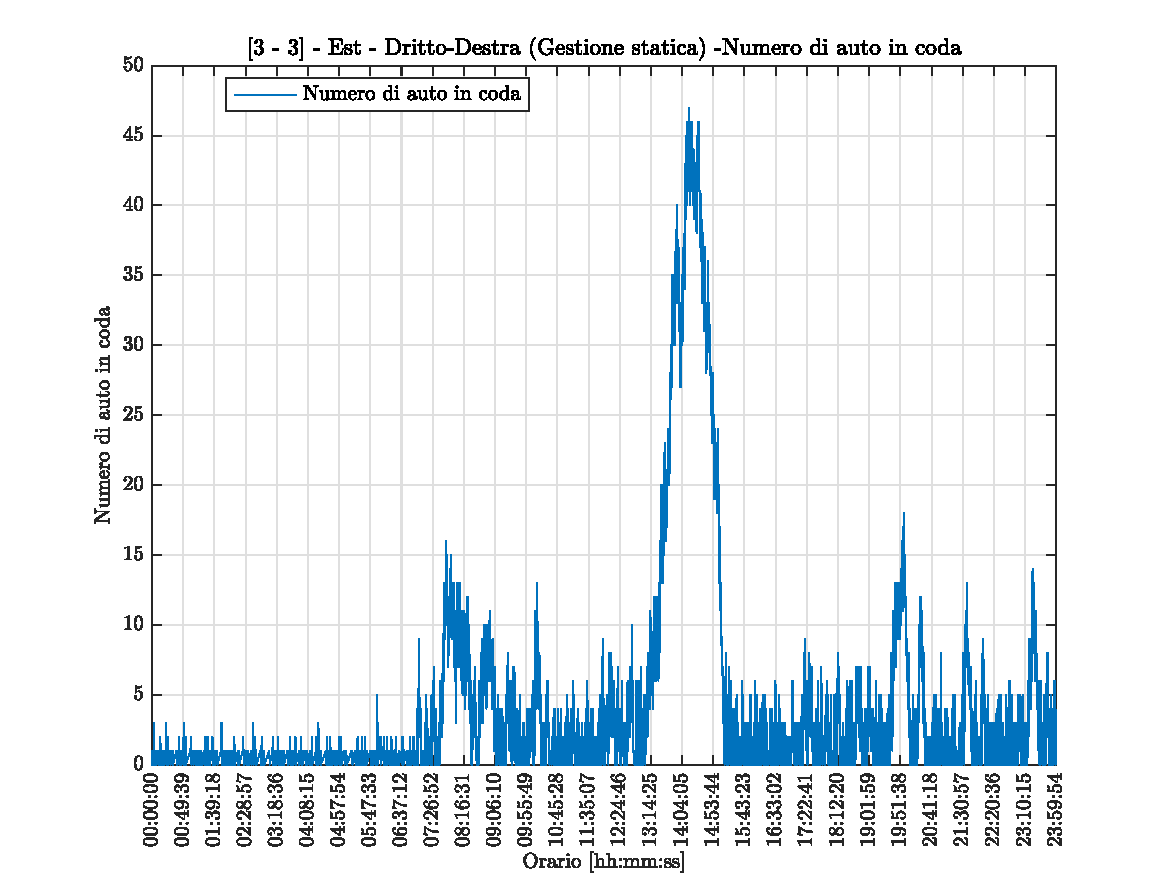
\includegraphics[width=0.9\textwidth]{autocodacap3.pdf}
  \caption{Variazione nel tempo del numero di auto in coda, corsia più congestionata della simulazione}
  \label{fig:}
\end{figure}
\begin{figure}[H]
\centering
  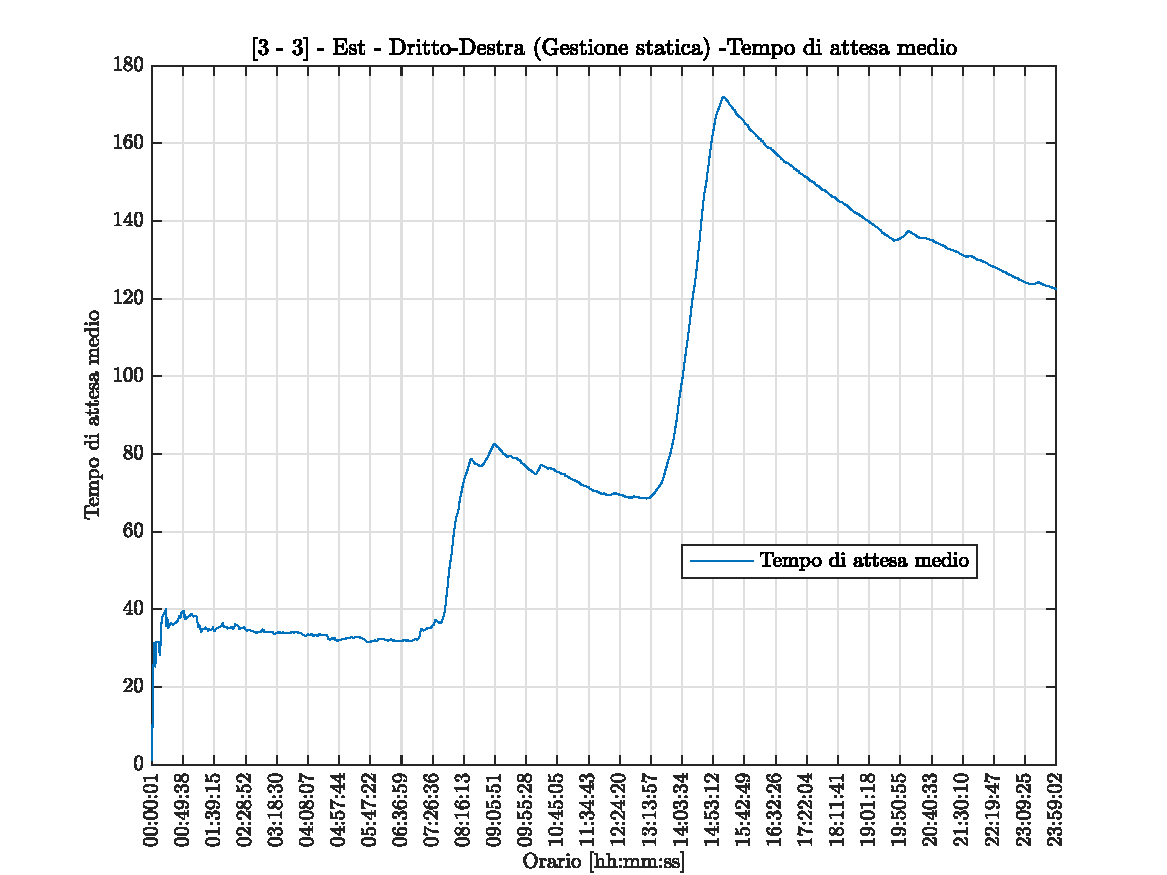
\includegraphics[width=0.9\textwidth]{tempoattesacap3.pdf}
  \caption{Tempi di attesa in funzione della fascia oraria, corsia più congestionata della simulazione}
  \label{fig:}
\end{figure}
\newpage

\begin{figure}[H]
\centering
  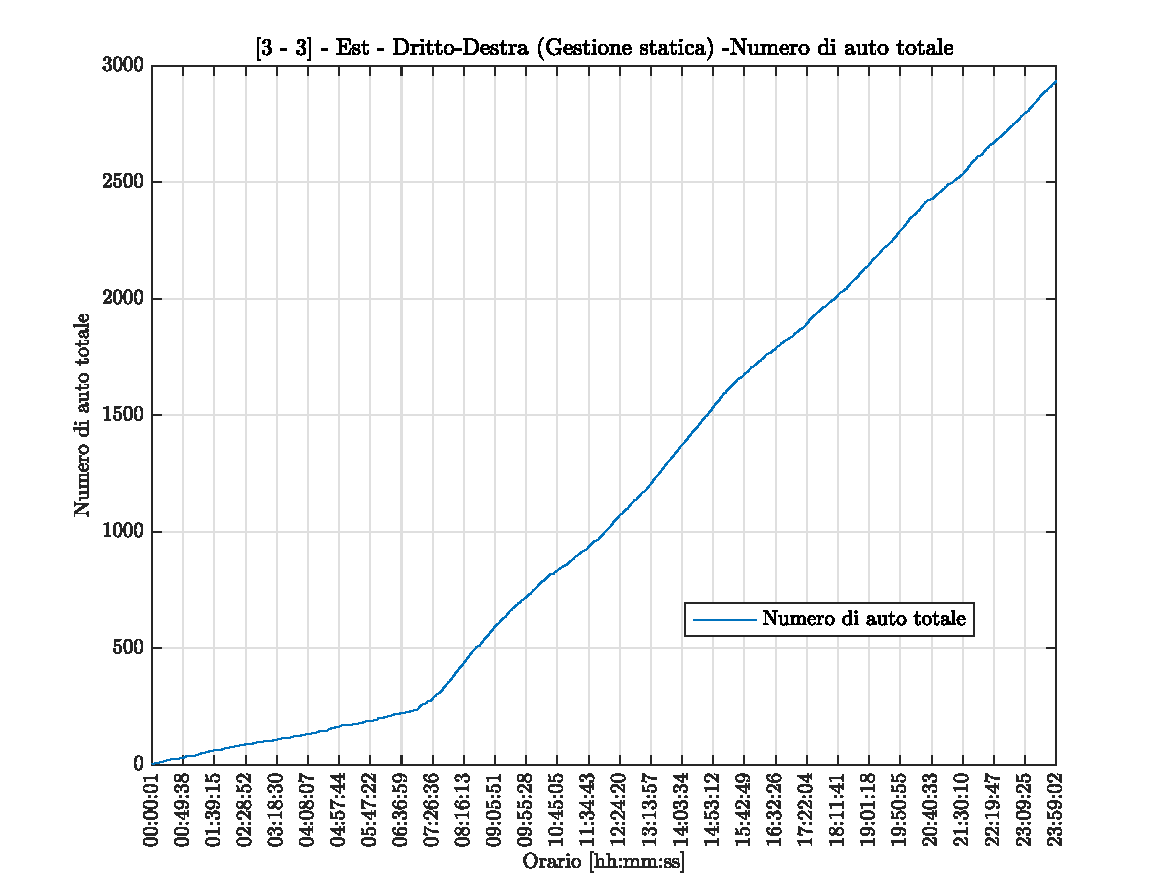
\includegraphics[width=0.9\textwidth]{autototcap3.pdf}
  \caption{Numero complessivo di auto, corsia più congestionata della simulazione}
  \label{fig:}
\end{figure}













